%\section{Discussion} \label{discussion}
%The model that achieved the highest F1 score on the validation set were MLP neural networks. The difference in accuracy and F1 score between the validation and test set was shown to be smaller in comparison to SVMs and random forest.

One qualitative advantage of using a random forest classifier is its training speed, which made hyperparameter tuning easier. The maximum number of levels in each decision tree was set to 80, the maximum number of features considered for splitting a node was set to 4, the minimum number of data points allowed in a leaf node was set to 4 and the number of trees that were in the classifier was set to 200.

Another significant advantage of a random forest classifier is that the importance of features can also be extracted and visualised.  \figref{fig4} shows this as the the mean decrease in Gini impurity for features across all trees. The impurity of a node is the probability of a specific feature being classified incorrectly assuming that it is selected randomly \cite{cassidy2014calculating}.

\begin{figure}[ht]

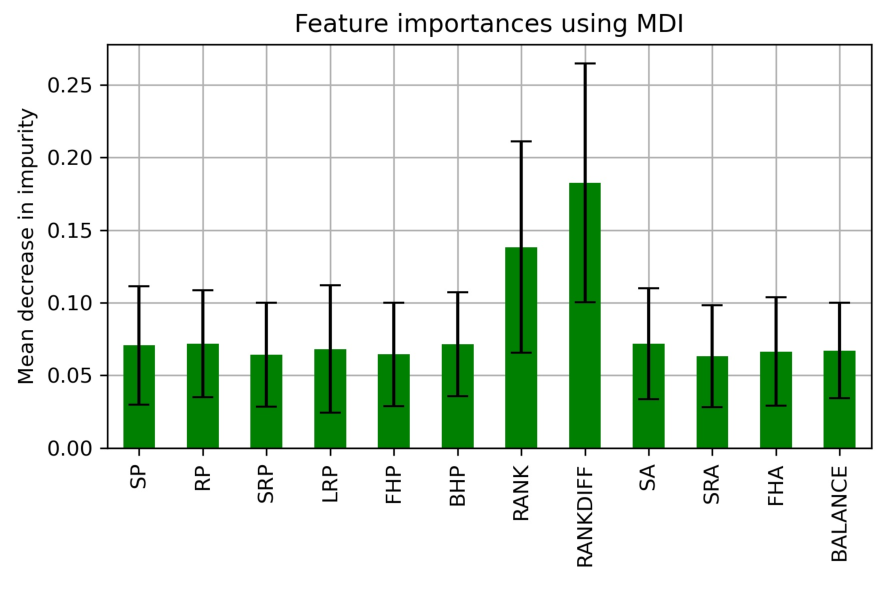
\includegraphics[width=8.5cm]{plots/feature_importance.pdf}
\caption{Importance of features from random forest classifier based on Gini impurity. In our dataset, RANKDIFF appears to be the most important feature.}
%\denes{Can we put * on the derived features, please?}. }
\vspace{-1em}
\label{fig:fig4}
\centering
\end{figure}

\subsection{Ablation Study}
\figref{fig4} predicts that the most important feature in a random forest model is  RANKDIFF, which justifies the inclusion of hand-crafted features. To reinforce this finding, we report the accuracy and F1 score for each model with and without the derived features (see \secref{engineer}). All scores are lower for models that don't use newly derived features, and accuracy score is significantly lower in SVMs compared to other models. Detailed results  are in Table \ref{results2}.

\begin{table}[ht]
\caption{Model performance with and without newly derived features}
\label{results2}
\centering
\setlength{\tabcolsep}{8pt}
\scalebox{1.05}{%
\begin{tabular}{ l|c c|c c }

\multirow{2}{4em}{Model} &
\multicolumn{2}{|c|}{With} &
\multicolumn{2}{|c}{Without} \\
\cline{2-5}
  & Acc & F1 & Acc & F1 \\

\hline \hline 
Logistic Regression & 0.699 & 0.705 & 0.631 & 0.668 \\
Random Forest & 0.677 & 0.688 & 0.661 & 0.673 \\
Support Vector Machine & & \\
$\rightarrow$ Linear & 0.696 & 0.690 & 0.556 & 0.619 \\
$\rightarrow$ RBF    & 0.700 & 0.677 & 0.500 & 0.591 \\
$\rightarrow$ Polynomial & 0.705 & 0.685 & 0.500 & 0.640\\
$\rightarrow$ Sigmoid & 0.705 & 0.690 & 0.472 & 0.642 \\
MLP Neural Network & 0.696 & 0.708 & 0.639 & 0.683\\
[1ex]
\hline
\end{tabular}}
\end{table}